\chapter{OPIS ROZWIĄZANIA}
\label{chapter:opis_rozwiazania}

\section{Architektura systemu}

System składa się z pięciu głównych komponentów: nadajników BLE (ang. \textit{BLE beacon}), aplikacji mobilnej, systemu Wit.ai, serwera oraz bazy danych. Grafikę przedstawiającą architekturę systemu można zobaczyć na rysunku \ref{fig:architecture}.

\begin{figure}[H]
    \centering
    \includesvg[width=\textwidth]{images/architecture.svg}
    \caption{Architektura systemu.}
    \label{fig:architecture}
\end{figure}

Aplikacja mobilna jest odpowiedzialna za odbieranie oraz przetwarzanie sygnału z nadajników. Jej zadaniem jest również interakcja z użytkownikiem i wysyłanie zapytań do serwera. Serwer przetwarza żądania użytkownika, wysyła zapytania do API (ang. \textit{Application Programming Interface}) serwisu Wit.ai, oraz komunikuje się z bazą danych. Baza danych przechowuje dane i modyfikuje lub udostępnia je na żadanie serwera. Komunikacja między aplikacją mobilną a serwerem odbywa się za pomocą protokołu HTTP. Serwer jest odpowiedzialny za przetwarzanie żądań użytkownika, a także za komunikację z bazą danych. Baza danych przechowuje dane o produktach, użytkownikach, koszykach, sklepach itp.

\section{Baza danych}

\subsection{Opis bazy danych}

Baza danych została zaimplementowana w PostgreSQL. Wybór tej bazy danych wynika z jej wszechstronności, wydajności oraz możliwości łatwego skalowania. Baza danych przechowuje informacje o produktach, użytkownikach, koszykach oraz sklepach. Schemat bazy danych przedstawia rysunek \ref{fig:database}.

Struktura bazy danych została zaprojektowana w sposób modularny, umożliwiając efektywne zarządzanie danymi dotyczącymi sklepów, użytkowników oraz produktów. Główną tabelą bazy danych jest tabela \textit{stores}, która przechowuje informacje o sklepach, takie jak nazwa, współrzędne geograficzne oraz miasto. Związek tej tabeli z tabelą \textit{sections} umożliwia podział sklepów na sekcje, które z kolei są przypisane do tabeli \textit{categories}, zawierającej dane o kategoriach produktów.

Produkty są przechowywane w tabeli \textit{products}, gdzie każdy rekord zawiera szczegóły takie jak nazwa, opis, cena, dostępność, ilość oraz jednostka miary, przechowywana w tabeli \textit{units}. Relacje między tabelami \textit{categories} i \textit{p}roducts pozwalają na przypisanie każdego produktu do konkretnej kategorii, co ułatwia organizację i wyszukiwanie danych.

Użytkownicy systemu są reprezentowani w tabeli \textit{users}, gdzie zapisywane są ich dane personalne, takie jak imię, nazwisko, adres e-mail oraz zaszyfrowane hasło. Każdy użytkownik może posiadać wiele koszyków zakupowych, co jest odzwierciedlone w tabeli \textit{carts}, przechowującej informacje o koszykach, takie jak data utworzenia i powiązanie z użytkownikiem. 
Szczegóły dotyczące zawartości koszyków są zapisane w tabeli \textit{cart\_items}, która łączy produkty z koszykami i zawiera informacje o liczbie sztuk danego produktu.

Relacje pomiędzy tabelami są realizowane za pomocą kluczy obcych, z zastosowaniem reguły ON DELETE CASCADE, co zapewnia integralność danych oraz automatyczne usuwanie powiązanych rekordów w przypadku usunięcia danych z tabel nadrzędnych. Taka organizacja umożliwia łatwe skalowanie bazy danych oraz wspiera utrzymanie spójności danych w systemie.

\begin{figure}[H]
    \includesvg[width=\textwidth]{images/database.svg}
    \caption{Schemat bazy danych.}
    \label{fig:database}
\end{figure}

\subsection{Szczegółowy opis tabel}

\subsubsection{Tabela stores}
\begin{itemize}
\item store\_id - SERIAL PRIMARY KEY: Unikalny identyfikator każdego sklepu.
\item store\_name - VARCHAR(255) NOT NULL: Nazwa sklepu.
\item latitude - VARCHAR(255) NOT NULL: Szerokość geograficzna określająca położenie sklepu.
\item longitude - VARCHAR(255) NOT NULL: Długość geograficzna określająca położenie sklepu.
\item city - VARCHAR(255) NOT NULL: Miasto, w którym znajduje się sklep.
\end{itemize}

\subsubsection{Tabela sections}
\begin{itemize}
\item section\_id - SERIAL PRIMARY KEY: Unikalny identyfikator sekcji sklepu.
\item section\_name - VARCHAR(255) NOT NULL: Nazwa sekcji w sklepie.
\item store\_id - INT REFERENCES stores(store\_id) ON DELETE CASCADE: Klucz obcy wskazujący sklep, do którego należy sekcja.
\end{itemize}

\subsubsection{Tabela categories}
\begin{itemize}
\item category\_id - SERIAL PRIMARY KEY: Unikalny identyfikator kategorii.
\item category\_name - VARCHAR(255) NOT NULL: Nazwa kategorii produktów.
\item section\_id - INT REFERENCES sections(section\_id) ON DELETE CASCADE: Klucz obcy wskazujący sekcję, do której przypisana jest kategoria.
\end{itemize}

\subsubsection{Tabela units}
\begin{itemize}
\item unit\_id - SERIAL PRIMARY KEY: Unikalny identyfikator jednostki miary.
\item unit\_name - VARCHAR(50) NOT NULL: Pełna nazwa jednostki miary (np. “kilogram”).
\item unit\_symbol - VARCHAR(10) NOT NULL: Skrót jednostki miary (np. “kg”).
\end{itemize}

\subsubsection{Tabela products}
\begin{itemize}
\item product\_id - SERIAL PRIMARY KEY: Unikalny identyfikator produktu.
\item name - VARCHAR(255) NOT NULL: Nazwa produktu.
\item description - TEXT: Opis produktu.
\item price - DECIMAL(10,2) NOT NULL: Cena produktu w formacie dziesiętnym (np. 123.45).
\item category\_id - INT REFERENCES categories(category\_id) ON DELETE CASCADE: Klucz obcy wskazujący kategorię, do której należy produkt.
\item availability - VARCHAR(50) NOT NULL: Status dostępności produktu (np. “w magazynie”).
\item amount - DECIMAL(10,2) NOT NULL: Ilość dostępna w magazynie.
\item unit\_id - INT REFERENCES units(unit\_id) ON DELETE CASCADE: Klucz obcy wskazujący jednostkę miary produktu.
\end{itemize}

\subsubsection{Tabela users}
\begin{itemize}
\item user\_id - SERIAL PRIMARY KEY: Unikalny identyfikator użytkownika.
\item email - VARCHAR(255) UNIQUE NOT NULL: Adres e-mail użytkownika.
\item password - VARCHAR(255) NOT NULL: Hasło użytkownika (w formie zaszyfrowanej).
\item first\_name - VARCHAR(50) NOT NULL: Imię użytkownika.
\item last\_name - VARCHAR(50) NOT NULL: Nazwisko użytkownika.
\end{itemize}

\subsubsection{Tabela carts}
\begin{itemize}
\item cart\_id - SERIAL PRIMARY KEY: Unikalny identyfikator koszyka.
\item user\_id - INT REFERENCES users(user\_id) ON DELETE CASCADE: Klucz obcy wskazujący użytkownika, do którego należy koszyk.
\item creation\_date - TIMESTAMP DEFAULT CURRENT\_TIMESTAMP: Data i czas utworzenia koszyka.
\end{itemize}

\subsubsection{Tabela cart\_items}
\begin{itemize}
\item cart\_item\_id - SERIAL PRIMARY KEY: Unikalny identyfikator pozycji w koszyku.
\item cart\_id - INT REFERENCES carts(cart\_id) ON DELETE CASCADE: Klucz obcy wskazujący koszyk, do którego należy pozycja.
\item product\_id - INT REFERENCES products(product\_id) ON DELETE CASCADE: Klucz obcy wskazujący produkt dodany do koszyka.
\item quantity - INT NOT NULL: Liczba sztuk danego produktu w koszyku.
\end{itemize}

tekst

\section{Interfejs użytkownika}

\subsection{Opis dostępnych widoków}

\subsubsection{Strona tytułowa}

\begin{center} 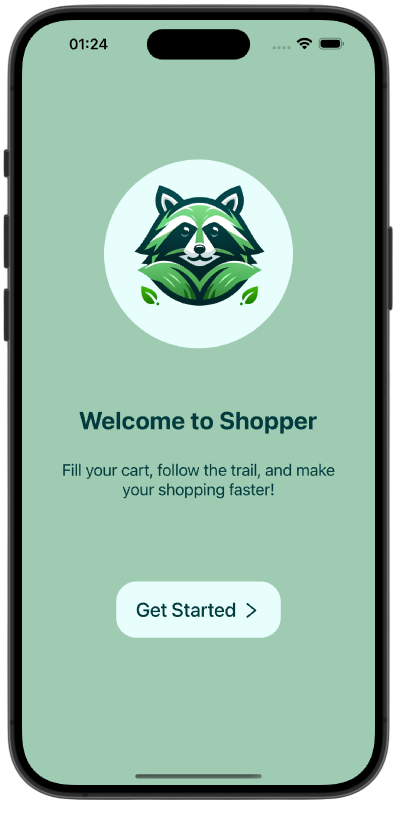
\includegraphics[width=0.4\textwidth]{images/front/home_page.png} \end{center}

Strona tytułowa aplikacji pełni funkcję ekranu startowego, witając odbiorcę logiem oraz hasłem zachęcającym do korzystania z aplikacji. Widnieje na niej przycisk "Get Started", który umożliwia przejście do kolejnych widoków. Jeśli eksploatator był zalogowany w ciągu ostatnich 7 dni, aplikacja przekierowuje go do widoku logowania. W przeciwnym wypadku trafia on do ekranu profilu. Całość utrzymana jest w przyjaznej stylistyce, z dominującym odcieniem zieleni oraz spójną paletą kolorów, wygenerowaną przez narzędzie DALL·E 3 od OpenAI.

\begin{center} 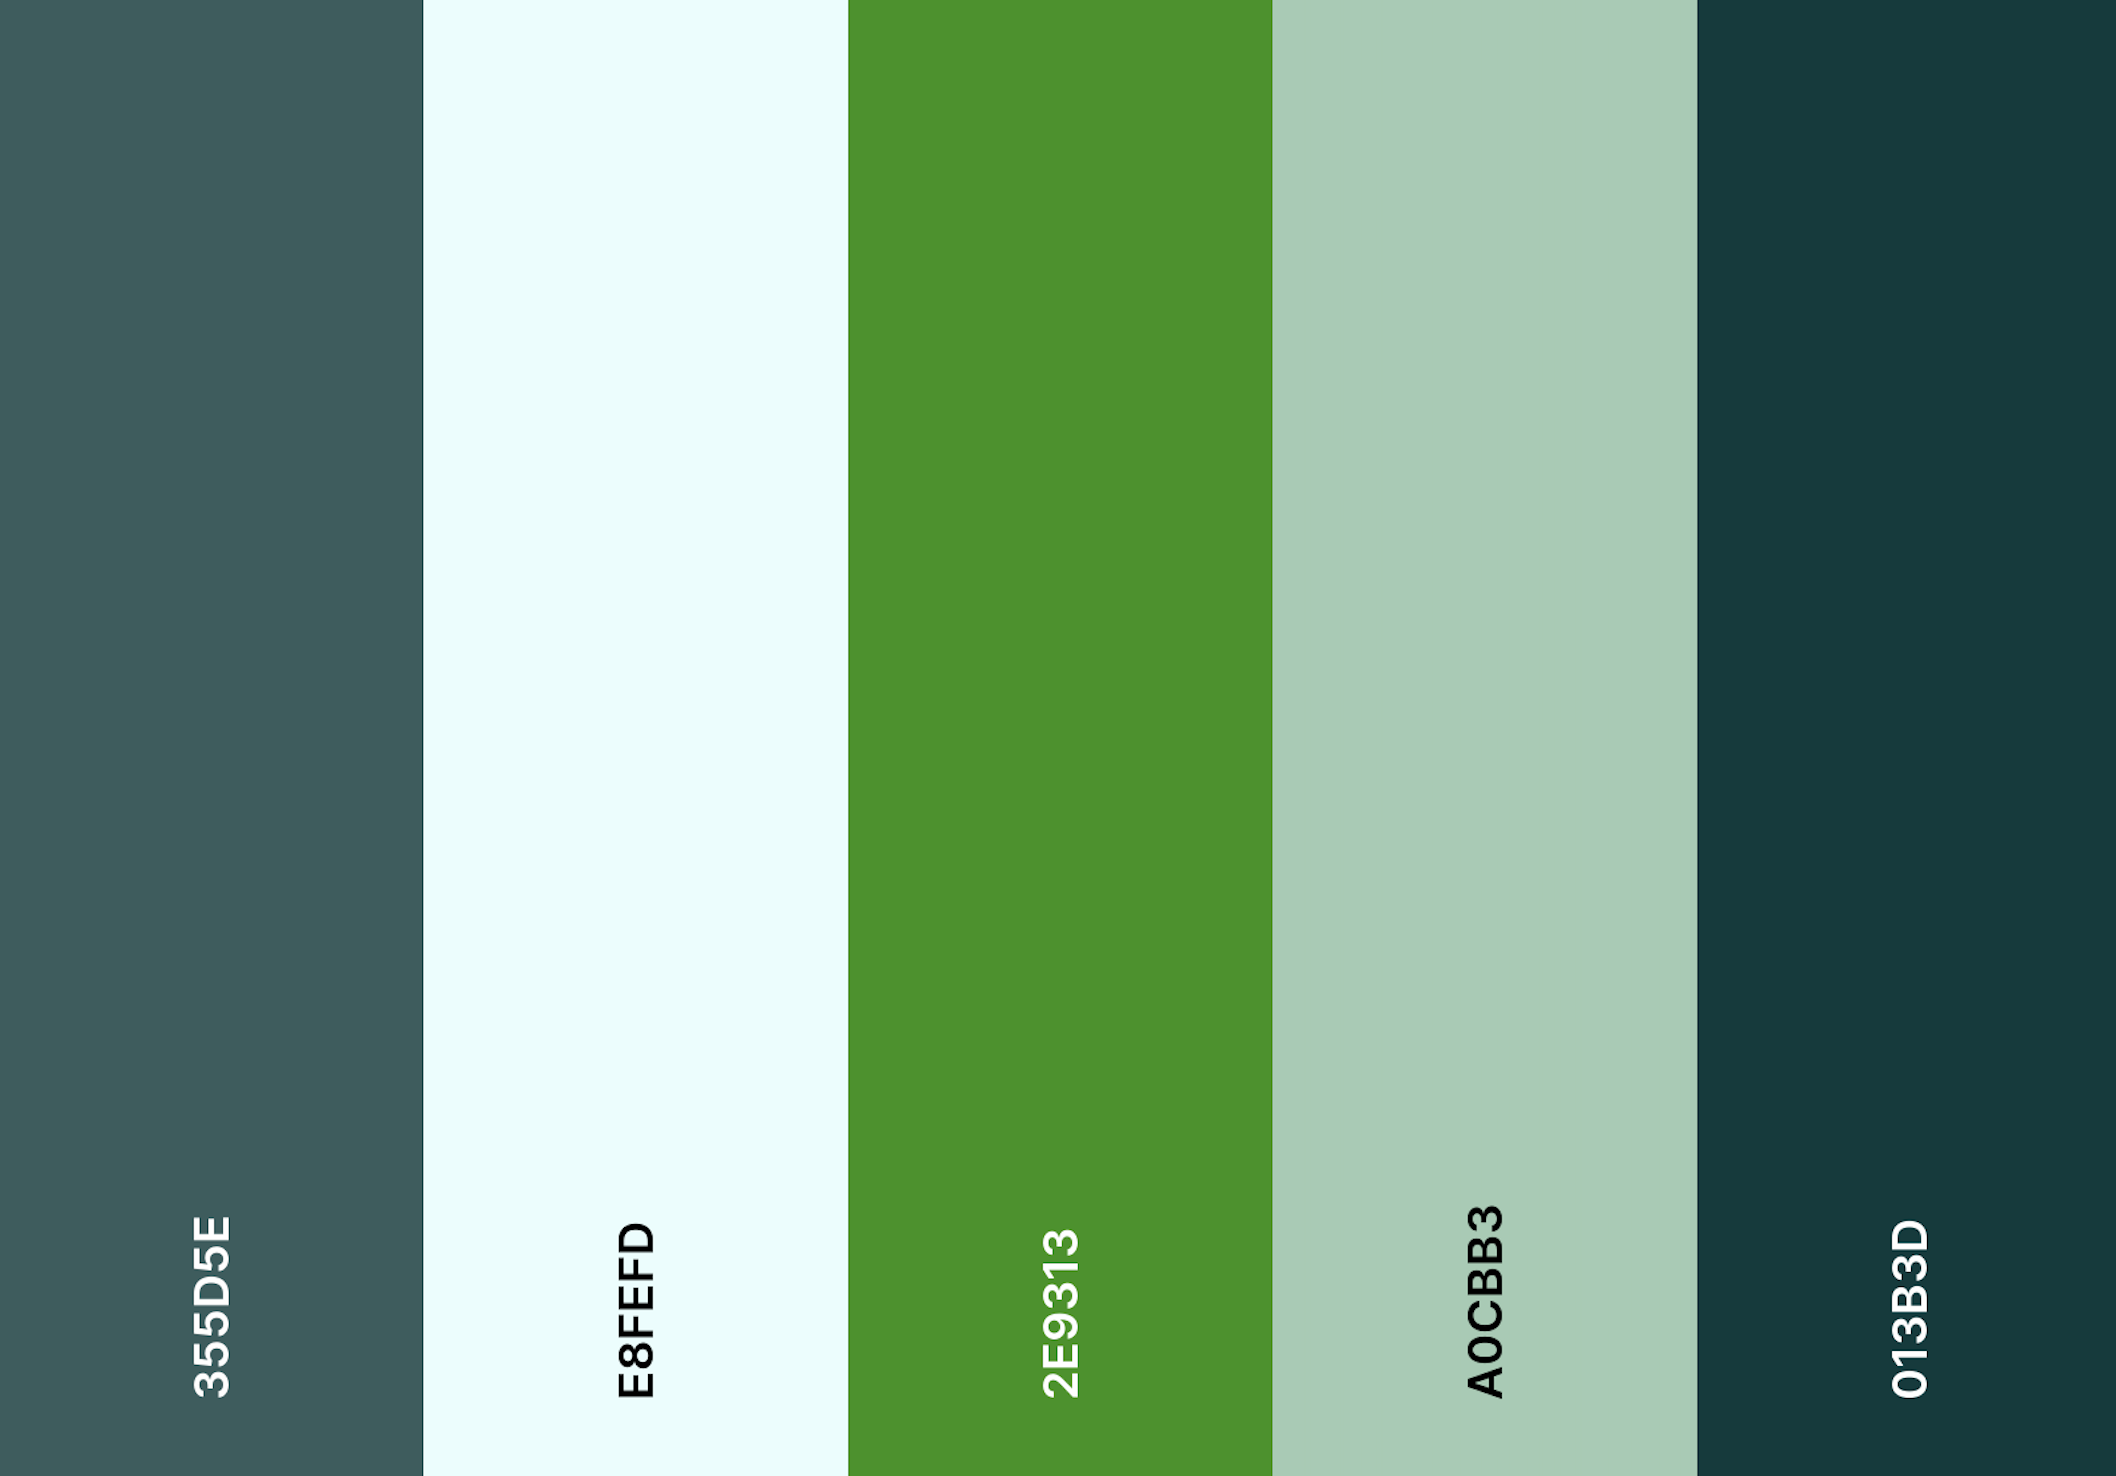
\includegraphics[width=0.6\textwidth]{images/front/theme.png} \end{center}

\subsubsection{Ekran logowania}

\begin{center} 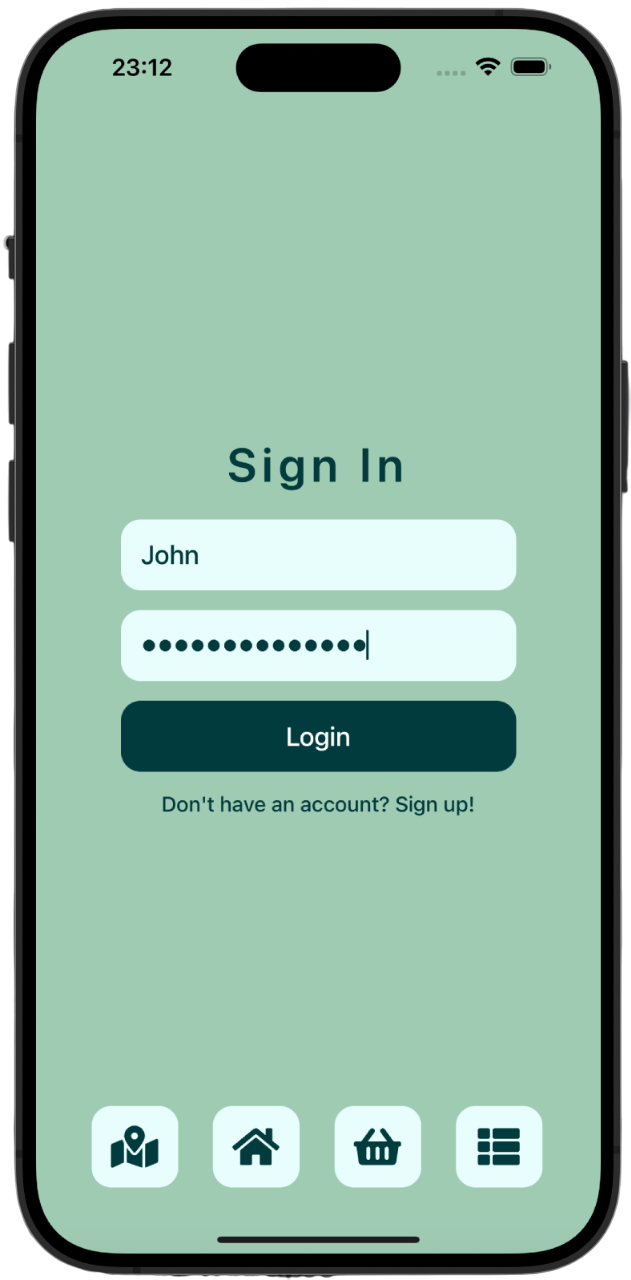
\includegraphics[width=0.4\textwidth]{images/front/login_page.png} \end{center}

Ekran logowania umożliwia odbiorcy uwierzytelnienie w aplikacji poprzez wprowadzenie adresu e-mail oraz hasła. Jego głównym celem jest weryfikacja tożsamości eksploatatora oraz przekierowanie do dalszych widoków w zależności od wyniku logowania. Górną część widoku stanowi nagłówek "Sign In", który podkreśla cel ekranu. Środkową część zajmuje formularz składający się z dwóch pól tekstowych: jednego przeznaczonego do wprowadzania adresu e-mail, a drugiego do hasła, z cechą ukrywania wprowadzanych znaków. Naciśnięcie przycisku "Login" uruchamia logikę, która weryfikuje tożsamość odbiorcy na podstawie danych wprowadzonych w polach tekstowych. Ponadto, widok zawiera link "Don't have an account? Sign up!", umożliwiający przejście do widoku rejestracji. Dolną część ekranu zajmuje pasek nawigacyjny z ikonami, które przenoszą do kolejnych podstron – mapy sklepów, profilu odbiorcy, kategorii produktów wybranego sklepu oraz strony tytułowej. Tylko ta ostatnia jest dostępna dla niezalogowanych użytkowników.

\subsubsection{Ekran rejestracji}

\begin{center} 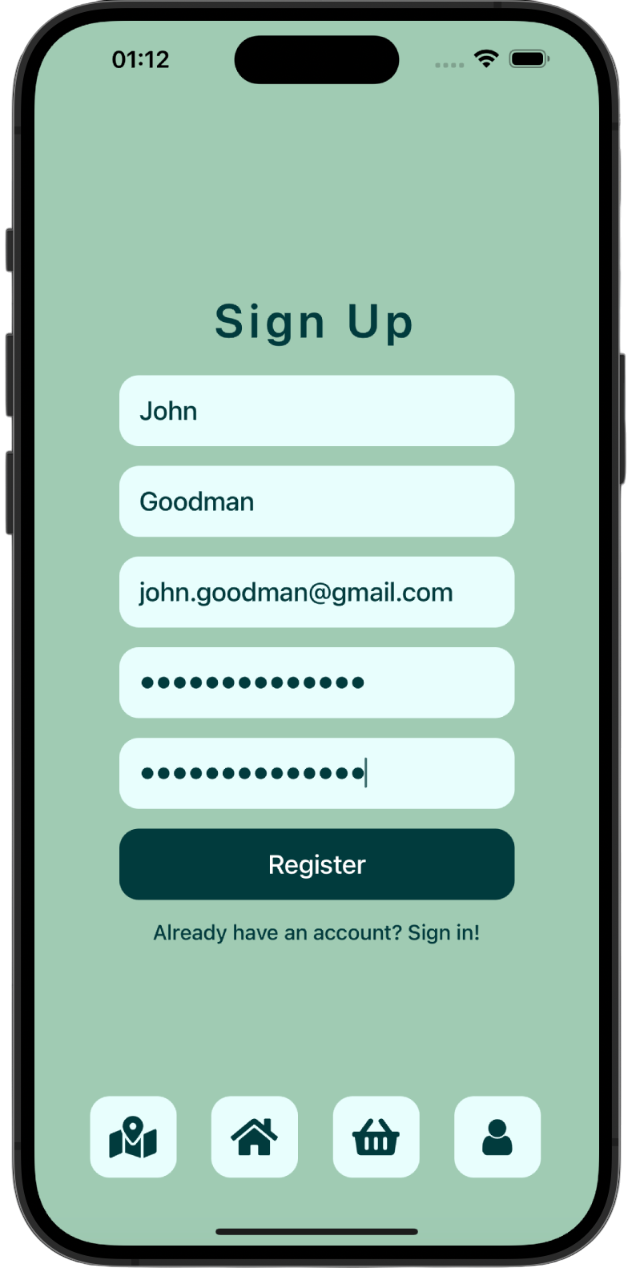
\includegraphics[width=0.4\textwidth]{images/front/register_page.png} \end{center}

Ekran rejestracji umożliwia nowym odbiorcom założenie konta, co jest niezbędne do korzystania z funkcji wymagających uwierzytelnienia, takich jak dodawanie produktów do koszyka czy przeglądanie sklepów na mapie. Formularz rejestracyjny składa się z kilku pól:

\begin{itemize} \item Firstname i Lastname – wymagane minimum trzech znaków, by dane były wystarczająco szczegółowe. \item Email – odbiorca podaje swój adres e-mail, który jest weryfikowany pod kątem poprawności formatu (obecność znaku "@" oraz domeny). \item Password i Repeat password – hasło musi mieć co najmniej osiem znaków i być identyczne w obu polach. Dodatkowo, tekst wprowadzony w tych polach jest ukrywany, aby zapewnić prywatność. \end{itemize}

Po wypełnieniu formularza, należy wcisnąć guzik "Register", po którym odbywa się walidacja danych. W przypadku spełnienia warunków wpisanych pól, nowy użytkownik, wraz z koszykiem jest rejestrowany w bazie danych. Po zakończeniu rejestracji następuje automatyczne zalogowanie, a imię oraz ID są zapisywane w lokalnej pamięci urządzenia, w bezpieczny sposób, aby dane nie trafiły w niepowołane ręce. Pozwala to na sprawne obslużenie mechanizmu sesji oraz dostępu do koszyka jego właściciela. Następnie następuje przekierowanie do ekranu kategorii produktów wybranego sklepu. Jeśli dane są nieprawidłowe, wyświetlane są stosowne komunikaty, informujące o błędach, takich jak niewłaściwy format e-maila, zbyt krótkie hasło czy jego niezgodność. Osoby posiadające już konto mogą skorzystać z linku "Already have an account? Sign in!", znajdującego się pod formularzem, aby przejść do ekranu logowania. Dolną część ekranu zajmuje pasek nawigacyjny, który zawiera przyciski prowadzące do kolejnych sekcji aplikacji. Pierwszy z nich przekierowuje do widoku mapy sklepów. Kolejny przekierowuje na stronę główną – jest to jedyny dostępny dla niezalogowanych odbiorców. Trzeci zawiera ikonę koszyka, w którym użytkownicy mogą przeglądać swoje produkty, a czwarty prowadzi do profilu odbiorcy, gdzie można zarządzać danymi konta.

\subsection{Szczegółowe omówienie implementacji}
\subsubsection{Strona tytułowa}